\documentclass{article}
\usepackage{graphicx} 
\usepackage{pgf-pie}
\usepackage[colorlinks=true, urlcolor=blue]{hyperref}

\title{Logistics : CS230 and CS231}
\date{}

\begin{document}

\maketitle

\section{Course Websites}
\subsection{CS230}
Course Information + Lecture Slides : \\\url{https://cs230-iitb.github.io/autumn-2026/}\\\\
Discussion Portal (Piazza) : \\\url{https://piazza.com/class/ms1a6g1fg1luv}
\subsection{CS231}
Labs : \\
\url{https://github.com/CS231-DLDCA-Lab/CS231-2026}
\\\\
Lab seat mapping : \\\url{https://docs.google.com/spreadsheets/d/1tayAATniMwQ7fh3_62BuHnNRad7Ltvios91gzEG3gZ0/edit?usp=sharing}
\section{Quizzes}

        \subsection{CS230}
        Theory Quiz 1 : September 1st Week
\newpage
\section{Grade Distribution}
\subsection{CS230 (Theory)}
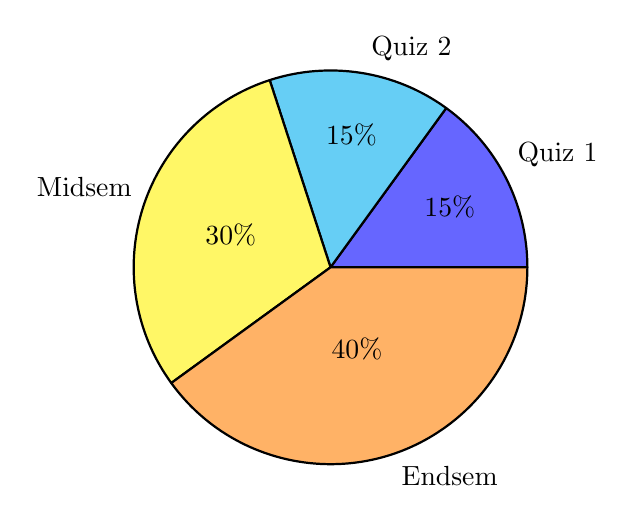
\begin{tikzpicture}
  \pie[radius=2.5]{15/Quiz 1, 15/Quiz 2, 30/Midsem, 40/Endsem}
\end{tikzpicture}
\subsection{CS231 (Lab)}
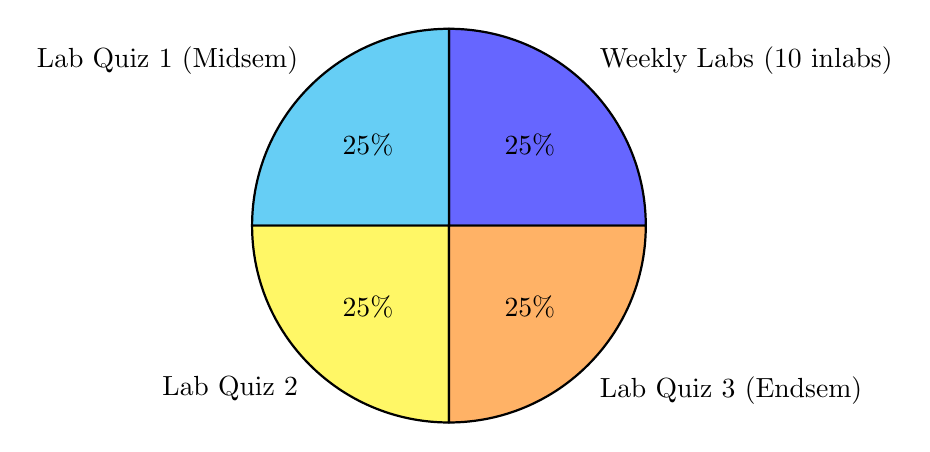
\begin{tikzpicture}
  \pie[radius=2.5]{25/Weekly Labs (10 inlabs), 25/Lab Quiz 1 (Midsem), 25/Lab Quiz 2, 25/Lab Quiz 3 (Endsem)}
\end{tikzpicture}



\end{document}
